% The two-stage flexible flow shop and the two operations of a job, as two pictures set side by side
% and centered on each other. Adapted from the slide "Problem Definition".
\begin{tikzpicture}[baseline=(current bounding box.center)]
\tikzset{mach/.style={circle,thick,draw,minimum size=0.62cm,inner sep=0pt,font=\footnotesize}}
% the shop: one first-stage machine feeding m identical second-stage machines
\node[mach,fill=red!25] (s) at (0,1.2) {};
\node[anchor=east,font=\footnotesize,align=right] at (-0.5,1.2) {first stage:\\one machine};
\node[mach,fill=yellow!35] (m1) at (-1.7,-0.9) {$1$};
\node[mach,fill=yellow!35] (m2) at (-0.55,-0.9) {$2$};
\node at (0.55,-0.9) {$\cdots$};
\node[mach,fill=yellow!35] (mm) at (1.7,-0.9) {$m$};
\foreach \t in {m1,m2,mm}
    \draw[-{Stealth[length=2.4mm]},line width=1pt] (s) -- (\t);
\node[font=\footnotesize] at (0,-1.7) {second stage: $m$ identical machines};
\end{tikzpicture}%
\hspace{1.4cm}%
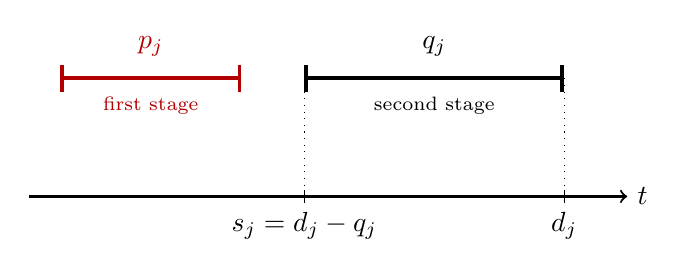
\begin{tikzpicture}[baseline=(current bounding box.center)]
\colorlet{prep}{red!70!black}
% the two operations of one job
\draw[->,thick] (-0.2,0) -- (7.4,0) node[right] {$t$};
\draw[|-|,line width=1.4pt,prep] (0.2,1.5) -- (2.5,1.5);
\node[prep] at (1.35,1.9) {$p_j$};
\node[prep,font=\scriptsize] at (1.35,1.15) {first stage};
\draw[|-|,line width=1.4pt] (3.3,1.5) -- (6.6,1.5);
\node at (4.95,1.9) {$q_j$};
\node[font=\scriptsize] at (4.95,1.15) {second stage};
\draw[dotted] (3.3,1.5) -- (3.3,0);
\draw[dotted] (6.6,1.5) -- (6.6,0);
\draw (3.3,0.08) -- (3.3,-0.08) node[below] {$s_j=d_j-q_j$};
\draw (6.6,0.08) -- (6.6,-0.08) node[below] {$d_j$};
\end{tikzpicture}
